%%%%%%%%%%%%%%%%%%%%%%%%%%%%%%%%%%%%%%%%%%%%%%%%%%%%%%%%%%%%%%%%%%%%%%%%%%%

\documentclass{standalone}

\usepackage{amsmath}
\usepackage{mathptmx}
\usepackage{tikz}
\usetikzlibrary{external}
\tikzexternalize{running-ants}

%% IEEE uses Times Roman font, so we'll default to Times.
%% These three commands make up the entire times.sty package.
\renewcommand{\rmdefault}{ptm}
\renewcommand{\ttdefault}{pcr}
\normalfont\selectfont

%%%%%%%%%%%%%%%%%%%%%%%%%%%%%%%%%%%%%%%%%%%%%%%%%%%%%%%%%%%%%%%%%%%%%%%%%%%
%% A rectangular region.
%%%%%%%%%%%%%%%%%%%%%%%%%%%%%%%%%%%%%%%%%%%%%%%%%%%%%%%%%%%%%%%%%%%%%%%%%%%

\begin{document}

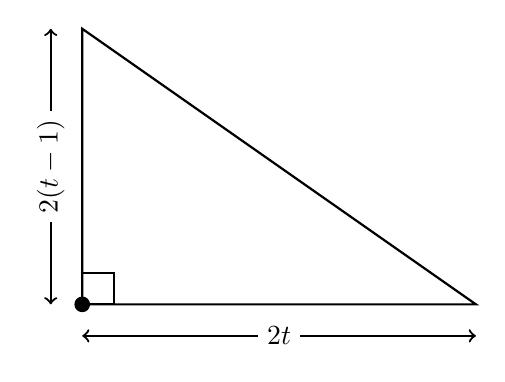
\begin{tikzpicture}[%%
  arrowStyle/.style={<->,thick},%%
  dotStyle/.style={circle,inner sep=2pt,black,fill=black},%%
  labelStyle/.style={fill=white},%%
  lineStyle/.style={-,thick}%%
]
%%
%%
\pgfmathsetmacro{\dx}{0.4}
\pgfmathsetmacro{\dy}{\dx}
\pgfmathsetmacro{\length}{5}
\pgfmathsetmacro{\width}{3.5}
\pgfmathsetmacro{\xlow}{0}
\pgfmathsetmacro{\ylow}{\xlow}
%%
\coordinate (eastRight) at (\length,\ylow);
\coordinate (northTop) at (\xlow,\width);
\coordinate (origin) at (\xlow,\ylow);
%%
\normalsize
%% Draw the triangle.
\draw[lineStyle] (eastRight) -- (origin) -- (northTop) -- cycle;
\draw[lineStyle] (origin) rectangle (\dx,\dx);
% %% Label the base of the triangle.
\draw[arrowStyle] (\xlow,-\dy) -- (\length,-\dy);
\node[labelStyle] at (\length/2,-\dy) {$2t$};
%% Label the height of the triangle.
\draw[arrowStyle] (-\dx,\ylow) -- (-\dx,\width);
\node[labelStyle,rotate=90] at (-\dx,\width/2) {$2(t - 1)$};
%% Label the starting point.
\node[dotStyle] at (origin) {};
\end{tikzpicture}

\end{document}
